%!TEX root=final_report_nips.tex
\section{Implementation}
The STEM data produced by eBird came in \texttt{Rdata} format. Thus, our first step is transforming that data into CSV format. We then read the data into Python where we generate the averaged time-series data for each bounding box (with the number of boxes as a parameter). 

Our network inference implementation then chooses a time-window of roughly 2 months and computes the cross-correlation for all candidate edges (which are the $8n$ 8-neighborhood edges noted above, minus any with incident nodes that have been filtered due to low population). We then perform the Fisher transformation of the correlations, and perform the significance test. Thus, the general process is as follows:

\begin{enumerate}
\item Filter out zero-population and low-action ($p_{active} < 0.05$) nodes
\item Compute spatially localized cross-correlations with lags $1\dots T, (T=10)$
\item Use significance test to determine if cross-correlations are statistically valid
\item Keep valid edges
\end{enumerate}

The edges generated for each time period are returned as a list of tuples which can then be plotted on a map.

\subsection{Filtering}
Given the large geographic coverage of the timeseries data, we had to employ several techniques to remove noise and control the density of edges returned by the inference.
Because the inference only leverages the cross correlation under a particular lag, we needed to employ more data about the movement of the species as well as the current species' density at a given node.
To better measure actual migration and not just co-presence, we employ three types of pre-filtering in our approach:
\begin{enumerate}
\item Zero-population -- all nodes that do not have any expected birds are immediately ignored.
\item Low-action ($p_{active} < 0.05$) nodes -- all nodes with very low bird occurrences are also removed to reduce the number of edges.  When there are two neighboring nodes with extremely low swallow presence we filter them to insure that the nodes on our migration paths are actually paths that many birds take. 
\item Stationary nodes -- time series derivative information is used to filter out the nodes that do not have movement.  Over each window we compute the average change in frequency for each location.  Low magnitude derivatives mean that the value of birds is stationary and no migration is occurring.  We leverage this directly to show only the migration structure and not just the presence.
\end{enumerate}


\section{Results}
We generated a graph of bird movement over each a series of 2-month windows created by rolling each window 2 weeks at a time.
The edges have transparency based on the average magnitude of the derivative, over the window, for both endpoints.
The underlying color represents the calculated bird presence from the data.
Edges with less movement--denoted by less change during the time window--will have considerably lighter colored edges in the graph.
The full series of generated graphs can be found in \ref{appendicks}.


\begin{figure}[ht]
\centering
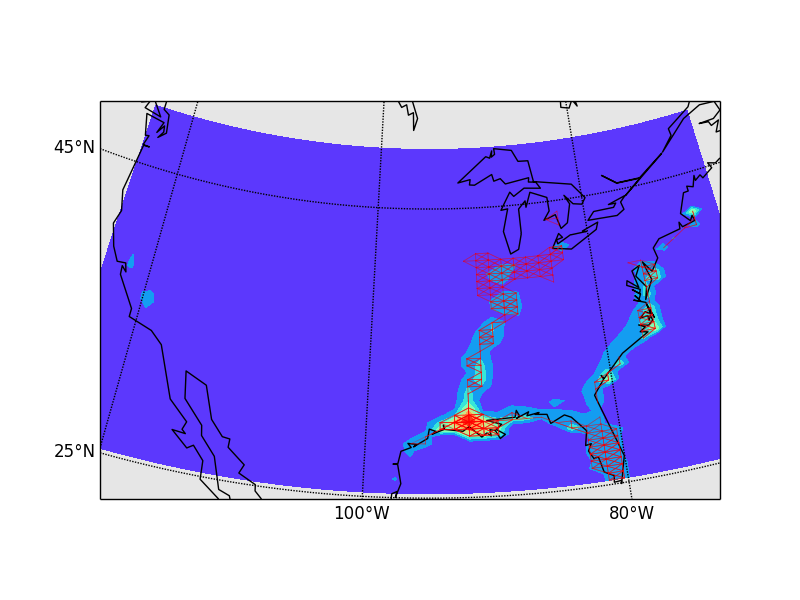
\includegraphics[width=.9\textwidth]{../code/swallowpics/bird38.png}
\caption{September through October the birds can be seen moving in two primary avenues, down the east coast flyway and down the Mississippi flyway.  Both routes are established migration patterns for many migratory species--including the treeswallow.}
\label{figBidLouisiana}
\end{figure}